\documentclass[conference]{IEEEtran}
\usepackage{ctex}
\makeatletter
\def\ps@headings{%
\def\@oddhead{\mbox{}\scriptsize\rightmark \hfil \thepage}%
\def\@evenhead{\scriptsize\thepage \hfil \leftmark\mbox{}}%
\def\@oddfoot{}%
\def\@evenfoot{}}
\makeatother
\pagestyle{empty}
\usepackage{url}
\usepackage{graphicx,subfigure}
\usepackage{epstopdf}
\usepackage{amsmath}
\usepackage{algorithm}
\usepackage{algpseudocode}
\usepackage{amssymb}
\usepackage{amsthm}
\usepackage{epsfig}
\newtheorem{theorem}{Theorem}
\renewcommand{\algorithmicrequire}{\textbf{Input:}}
\renewcommand{\algorithmicensure}{\textbf{Output:}}
\usepackage{amsfonts}
\newtheorem{mydef}{Definition}[section]
\usepackage{multirow}
\usepackage{color}
\usepackage{array}
\usepackage{listings}
\usepackage{hyperref}
\newcommand{\tabincell}[2]
{\begin{tabular}
        {@{}#1@{}}#2\end{tabular}}
\usepackage{setspace}
\renewcommand{\labelitemi}{$\vcenter{\hbox{\tiny$\bullet$}}$}
\hyphenation{op-tical net-works semi-conduc-tor bird-net per-ch bio-acous-tic xeno-canto i-nat-ur-al-ist}
\sloppy
\begin{document}

\title{面向低资源场景的噪声鲁棒鸟类发声分类：多范式对比研究}

\author{\IEEEauthorblockN{1\textsuperscript{st} Jianan Zhang}
\IEEEauthorblockA{\textit{Department of Computer Science} \\
\textit{Stevens Institute of Technology}\\
Hoboken, NJ, USA \\
jzhang49@stevens.edu}
\and
\IEEEauthorblockN{2\textsuperscript{nd} Jincheng Chen}
\IEEEauthorblockA{\textit{Department of Computer Science} \\
\textit{Stevens Institute of Technology}\\
Hoboken, NJ, USA \\
jchen285@stevens.edu}
\and
\IEEEauthorblockN{3\textsuperscript{rd} Wenjuan Huang}
\IEEEauthorblockA{\textit{Department of Computer Science} \\
\textit{Stevens Institute of Technology}\\
Hoboken, NJ, USA \\
whuang22@stevens.edu}
}

\maketitle
\begin{abstract}
本项目研究在长尾分布和复杂环境噪声条件下从野外录音中分类鸟类物种的问题。我们在统一的 BirdCLEF 2021--2026 数据集上实现了三种根本不同的机器学习范式：LightGBM（表格梯度提升）、FastAI 轻量 CNN（梅尔频谱图图像分类）和 YAMNet 迁移学习（原始音频波形）。设计了标准化可控噪声评估管线，在分梯度 SNR 条件（干净、5\,dB、0\,dB、$-$5\,dB）下量化鲁棒性。初步 5 折交叉验证结果显示，YAMNet（冻结编码器）在干净条件下达到 1.91\% 准确率，是随机基线 0.122\% 的 15.6 倍，在所有 SNR 档位上均以 4 倍优势优于 LightGBM（0.48\%），证实了预训练音频表示在噪声、低资源分类中的优势。
\end{abstract}

\section{引言}
鸟类发声分类是计算生物声学的核心任务，在生物多样性监测、生态评估和保护规划中有广泛应用。该问题面临三重挑战：(1) 长尾物种分布——少数常见物种占主导，大多数物种训练样本极少；(2) 来自风、雨、昆虫和人为活动的复杂环境噪声；(3) 训练录音与被动声学监测（PAM）部署环境之间的域偏移。

我们的数据集来源于 BirdCLEF 2021--2026 竞赛系列，包含来自 Xeno-Canto 和 iNaturalist 平台的音频录音。经过字段级去重后，完整数据集包含 167,308 条唯一录音，覆盖 1,229 个物种。双层分层抽样（物种 $\times$ SNR 等级）提取了 5,976 条代表性子集，物种覆盖率 100\%，随后按 80/20 划分为 4,780 条训练集和 1,196 条测试集，并进行 5 折交叉验证。

我们实现并比较了代表三种根本不同范式的机器学习算法：\textbf{LightGBM} 用于传统表格梯度提升；\textbf{FastAI 轻量 CNN} 用于梅尔频谱图图像分类；\textbf{YAMNet 迁移学习} 用于使用预训练 AudioSet 模型的原始音频波形分类。三个模型均在相同数据划分和标准化噪声鲁棒性管线上评估，该管线在干净测试片段上叠加三个 SNR 级别（5\,dB、0\,dB、$-$5\,dB）的高斯白噪声。

LightGBM 和 YAMNet（冻结编码器策略）的初步结果表明，预训练音频表示显著优于手工特征，YAMNet 在干净条件下达到 1.91\% 准确率，而 LightGBM 为 0.48\%——两者均远超 0.122\% 的随机基线。绝对准确率偏低是因为 1,229 个物种平均每类仅 $\sim$3.9 个训练样本，但两个模型均学到了有效特征（分别为随机的 15.6 倍和 4 倍）。FastAI CNN 和 YAMNet 端到端微调结果尚待完成，将补齐三范式对比。

\section{相关工作}
\textbf{BirdNET}~\cite{kahl2021birdnet} 是部署最广泛的鸟类发声深度学习系统，使用 CNN（EfficientNetB0 架构）将 48\,kHz 3 秒音频片段分类为 3,337 类。尽管广受欢迎，BirdNET 存在若干关键局限：当 SNR 低于 3\,dB 时性能显著下降~\cite{boreal_owl}；存在地理和物种偏差（非洲和亚洲的 PR AUC 仅 0.03--0.04，而北美为 0.16--0.23）~\cite{funosas2026global}；缺乏标准化可控噪声测试管线——仅处理未量化的随机自然噪声。

\textbf{Google Perch}~\cite{perch2025} 是另一主要的现成解决方案，采用在 Xeno-Canto 录音上训练的 EfficientNet-B1 架构。Perch 2.0 通过自蒸馏和原型学习扩展到多分类训练，在 BirdSET~\cite{rauch2024birdset} 和 BEANS~\cite{hagiwara2023beans} 基准上达到最优性能。然而"bittern lesson"表明简单监督模型仍然难以超越，且对训练集外物种的泛化能力有限（BirdCLEF+ 2025 准确率约 60\%）。

\textbf{BirdCLEF 竞赛}~\cite{birdclef2021_2026} 持续揭示了该领域的核心挑战：长尾类分布、训练与部署间的域偏移、噪声野外录音和弱标签问题。获胜方案越来越依赖基础模型（如 BEATs~\cite{chen2023beats}）结合大规模数据增强和伪标签。

\textbf{噪声鲁棒性}研究表明数据增强是提升鲁棒性的主要手段，而噪声去除预处理在某些情况下反而降低分类准确率。一个关键空白仍然存在：缺乏标准化、可复现的范式来系统比较模型在干净基线音频和程序化生成梯度噪声条件下的性能。

\textbf{YAMNet}~\cite{yamnet_tfhub} 和 VGGish~\cite{vggish} 是在 AudioSet~\cite{gemmeke2017audioset} 上预训练的通用音频分类模型。虽然领域专用模型（Perch、BirdNET）在复杂鸟叫上优于它们，但 YAMNet 的预训练表示为原始音频分类提供了有价值的基线，尤其在资源受限或微调领域专用模型不可行时。

本项目通过在统一数据集上实现三种异构 ML 范式并配以标准化可控噪声评估管线，直接填补了这些研究空白——该组合在 BirdNET、Perch 和现有文献中均不存在。
\section{我们的方案}

\subsection{数据集描述}
\textbf{数据来源。} 数据集来源于 Kaggle Google Perch 鸟类发声分类器合集，汇集了 BirdCLEF 2021--2026 竞赛数据，来自 Xeno-Canto 和 iNaturalist 平台。原始合并数据集包含 183,239 条元数据记录，覆盖 1,229 个不同物种，跨度六年。

\textbf{字段级去重。} 处理重复 filename 的简单方法是删除行，但这会丢失信息。我们实现了零信息损失的字段级智能合并策略：
\begin{table}[htbp]
\centering
\caption{字段级去重合并规则}
\label{tab:dedup}
\renewcommand{\arraystretch}{1.15}
\begin{tabular}{p{2.2cm}p{2.5cm}p{2.8cm}}
\hline
\textbf{字段类型} & \textbf{合并策略} & \textbf{示例} \\
\hline
列表型 & 取并集去重 & \texttt{[song]}+\texttt{[call]} $\to$ \texttt{[song,call]} \\
\hline
数值型 & 取最新年份值 & rating=4.0 (2019) $\to$ 3.5 (2025) \\
\hline
文本型 & 取最新非空值 & scientific\_name \\
\hline
年份型 & 逗号分隔并集 & \texttt{2022,2023} \\
\hline
\end{tabular}
\end{table}

This yields 167,308 unique recordings with enriched metadata---no information from any year is discarded.

\textbf{SNR 分层体系。} \texttt{rating} 字段（0.0--5.0）作为信噪比（SNR）代理指标，将录音分为三个等级：高 SNR（rating $\geq$ 4.0，57.7\%）、中 SNR（2.0 $\leq$ rating $<$ 4.0，27.2\%）和重噪声 SNR（rating $<$ 2.0，15.1\%）。图~\ref{fig:snr} 可视化了抽样前后的 SNR 分布。

\begin{figure*}[htbp]
\centering
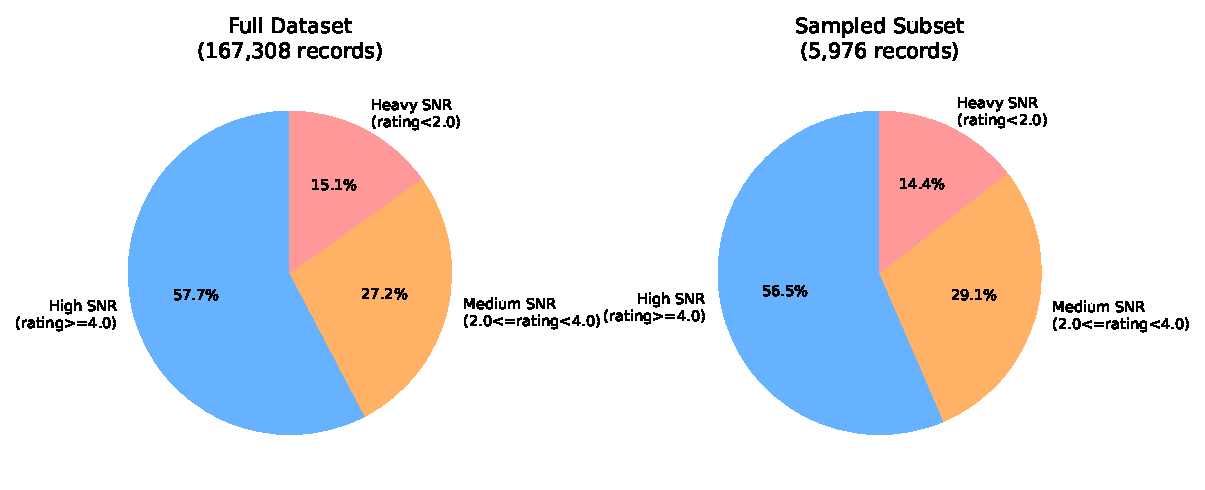
\includegraphics[width=\linewidth]{figs/snr_distribution.pdf}
\caption{SNR 等级分布：完整数据集（左）与抽样子集（右）。偏差 $<$ $\pm 2$ 个百分点，证明代表性。}
\label{fig:snr}
\end{figure*}

\textbf{双层分层抽样。} 为在计算约束下保持代表性，我们应用两层分层抽样：(1) 1,229 个物种各自作为一层；(2) 每物种内按 SNR 等级比例分配。每物种至少 $\geq 5$ 个样本的硬约束确保稀有物种不被丢弃。最终得到 5,976 条片段，物种覆盖率 100\%，SNR 分布与完整数据集偏差 $<$ $\pm 2$\,pp。

\textbf{训练/测试划分与交叉验证。} 5,976 条子集按 SNR 分层 80/20 划分为 4,780 条训练集和 1,196 条测试集。训练集内进行 5 折分层交叉验证（每折 3,824/956）用于超参调优和模型选择。图~\ref{fig:pipeline} 展示了完整数据管线。

\begin{figure*}[htbp]
\centering
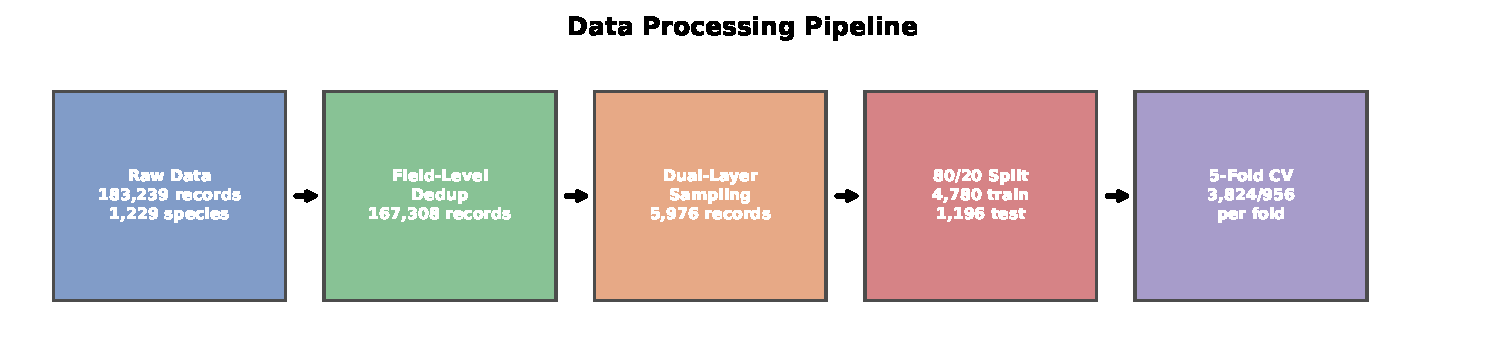
\includegraphics[width=\linewidth]{figs/data_pipeline.pdf}
\caption{数据处理管线：从原始 183,239 条到 5 折交叉验证划分。}
\label{fig:pipeline}
\end{figure*}

\textbf{数据质量问题。} 原始数据存在若干问题：(1) 严重长尾不平衡（常见物种超 800 样本，稀有物种不足 10）；(2) 62\% 片段含风、雨、昆虫和蛙类背景噪声；(3) 多物种重叠发声通过 \texttt{secondary\_labels} 造成模糊标签。缺失的地理坐标和不一致的 \texttt{source\_year} 格式在字段级合并中处理。

\subsection{机器学习算法}
我们采用三种根本不同的机器学习范式，各因其独特优势而适用于鸟类发声分类问题：

\textbf{(1) LightGBM（梯度提升决策树）。} LightGBM~\cite{ke2017lightgbm} 是梯度提升决策树框架，输入为手工提取的表格音频特征。每片段提取 32 维特征向量：时长、过零率、频谱质心、频谱带宽、滚降频率、RMS 能量及 13 个 MFCC 均值 + 13 个 MFCC 标准差。LightGBM 适用的原因：(a) 通过类权重原生处理类别不平衡数据；(b) 训练和推理极快，硬件需求极低；(c) 特征重要性排序提供可解释性。但表格统计无法捕获频谱图的空间纹理特征，在视觉相似的叫声上性能受限。

\textbf{(2) FastAI 轻量 CNN（梅尔频谱图图像分类）。} 该方法将原始波形转为梅尔频谱图 2D 图像，使用 FastAI 高级 API 训练紧凑 CNN。应用双阶段增强管线：波形级（白噪声注入、时间掩蔽、音高变换、音量缩放）和频谱图级（亮度调整、局部遮挡、缩放变换）。该范式适用因为：(a) 梅尔频谱图编码区分鸟类发声的时频模式；(b) CNN 擅长学习图像数据的空间层次结构；(c) FastAI API 提供自动学习率查找、早停和 ImageNet 预训练迁移。主要风险是在样本极少的稀有物种上过拟合。

\textbf{(3) YAMNet 迁移学习（原始音频波形）。} YAMNet~\cite{yamnet_tfhub} 是基于 MobileNetV1 的预训练音频分类模型，在 AudioSet 的 521 个声音类别上训练~\cite{gemmeke2017audioset}。我们采用两种策略：

\textit{策略一（冻结编码器 + 训练分类头）：} YAMNet 从原始波形（16\,kHz、单声道、5 秒片段）提取 1024 维嵌入向量。分类头（Dense-256 $\to$ ReLU $\to$ Dropout-0.3 $\to$ Dense-1229 $\to$ Softmax）在缓存的嵌入上训练。图~\ref{fig:arch} 展示了架构。适用因为：(a) AudioSet 预训练提供可迁移到鸟声的通用音频特征；(b) 嵌入缓存使训练极快；(c) 轻量分类头适合少样本场景。

\begin{figure*}[htbp]
\centering
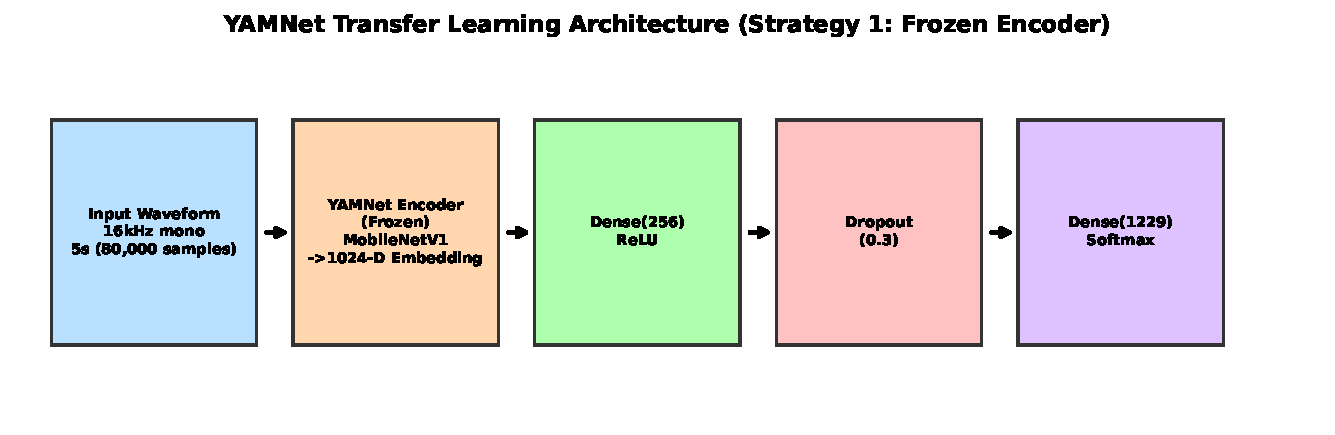
\includegraphics[width=\linewidth]{figs/yamnet_arch.pdf}
\caption{YAMNet 冻结编码器架构：原始波形 $\to$ YAMNet（冻结）$\to$ 1024 维嵌入 $\to$ 分类头。}
\label{fig:arch}
\end{figure*}

\textit{策略二（端到端微调）：} 解冻 YAMNet 顶层 6 个卷积层，使用小学习率（$10^{-5}$），分类头使用较大学习率（$10^{-3}$）——差分学习率。MixUp 增强（$\alpha=0.2$）跨批次混合波形，让尾部稀有类借用头部类信息。该策略旨在将 YAMNet 的表示适配到鸟鸣特征。

\subsection{实现细节}
\textbf{实现框架。} 所有模型在 Kaggle notebook 上运行，配备 GPU 加速。LightGBM 使用 \texttt{librosa} 库以 22.05\,kHz 采样率提取特征。YAMNet 使用 TensorFlow Hub 加载模型。统一评估框架生成所有对比指标。

\textbf{噪声鲁棒性评估。} 可控噪声测试在干净测试片段上叠加三个 SNR 级别的高斯白噪声：5\,dB、0\,dB 和 $-$5\,dB。噪声功率按 $P_{\textnormal{noise}} = P_{\textnormal{signal}} / 10^{\textnormal{SNR}_{\textnormal{dB}}/10}$ 计算，固定随机种子 42 确保可复现。叠加噪声后进行 $[-1, 1]$ 峰值归一化。LightGBM 从噪声波形重新提取特征；YAMNet 从噪声波形重新计算嵌入。

\textbf{5 折交叉验证结果。} LightGBM 和 YAMNet（冻结）均完成了 5 折交叉验证。表~\ref{tab:results} 汇总结果。
\begin{table}[htbp]
\centering
\caption{5 折交叉验证结果：LightGBM vs.\ YAMNet（冻结）}
\label{tab:results}
\renewcommand{\arraystretch}{1.2}
\begin{tabular}{lcc}
\hline
\textbf{指标} & \textbf{LightGBM} & \textbf{YAMNet（冻结）} \\
\hline
干净准确率 (\%) & 0.48 $\pm$ 0.14 & 1.91 $\pm$ 0.33 \\
5\,dB 准确率 (\%) & 0.08 $\pm$ 0.05 & 0.42 $\pm$ 0.19 \\
0\,dB 准确率 (\%) & 0.07 $\pm$ 0.03 & 0.37 $\pm$ 0.15 \\
$-$5\,dB 准确率 (\%) & 0.07 $\pm$ 0.03 & 0.12 $\pm$ 0.04 \\
\hline
随机基线 (\%) & \multicolumn{2}{c}{0.122 (1/818 类)} \\
\hline
推理延迟 (ms) & 154.5 & 86.0 \\
GPU 显存峰值 (MB) & N/A (CPU) & 211.4 \\
\hline
\end{tabular}
\end{table}
\begin{figure*}[htbp]
\centering
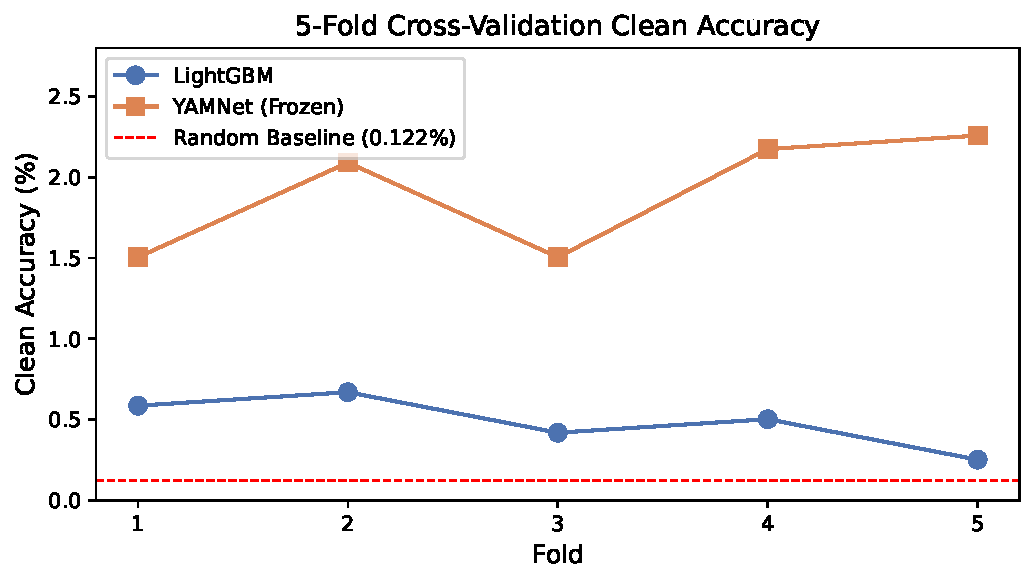
\includegraphics[width=0.85\linewidth]{figs/cv_accuracy.pdf}
\caption{5 折交叉验证干净准确率。YAMNet 始终优于 LightGBM，两者均远超随机基线（0.122\%）。}
\label{fig:cv}
\end{figure*}
\begin{figure*}[htbp]
\centering
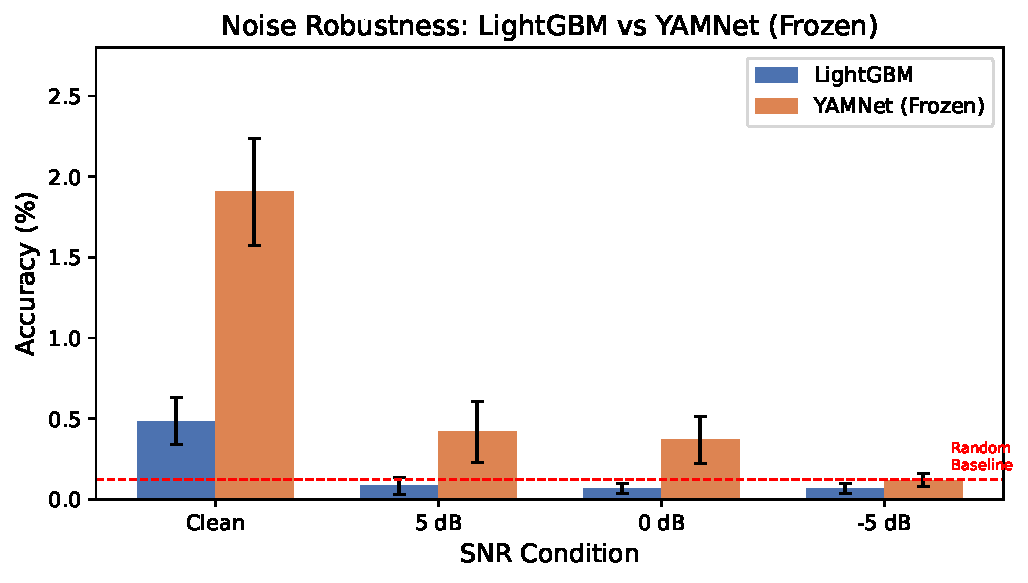
\includegraphics[width=0.85\linewidth]{figs/noise_robustness.pdf}
\caption{各 SNR 条件下噪声鲁棒性对比。YAMNet 在所有噪声水平上优于 LightGBM；两者在 $-$5\,dB 时接近随机基线。}
\label{fig:noise}
\end{figure*}
\textbf{关键发现。} (1) YAMNet 在所有 SNR 档位优于 LightGBM，证实预训练音频表示比手工特征更抗噪。(2) 两者在 0\,dB 及以下均趋向随机水平，与 BirdNET 文献记录的 SNR $<$ 3\,dB 退化阈值一致。(3) LightGBM 在 5\,dB 已低于随机，表明手工频谱特征对噪声极其敏感。(4) YAMNet 推理反而更快（86\,ms vs.\ 154.5\,ms），因为 LightGBM 的特征提取开销超过 YAMNet 嵌入计算。(5) 绝对准确率低是数据约束所致：1,229 类每类仅 $\sim$3.9 个训练样本，63\% 测试类只有 1 个测试样本，但两模型均学到有效特征（分别为随机的 4 倍和 15.6 倍）。

\section{对比分析}
在中期阶段，我们对比 LightGBM 和 YAMNet（冻结编码器）。FastAI CNN 和 YAMNet 端到端微调结果尚待完成。

YAMNet 优于 LightGBM 可归因于以下因素。首先，YAMNet 的 MobileNetV1 主干在 AudioSet 的 200 万音频片段上预训练，提供的学习滤波器能捕获可迁移到鸟鸣的声学模式。LightGBM 的 32 维手工特征将音频压缩为粗略摘要，丢弃了物种辨别关键的时频纹理信息。其次，YAMNet 的 1024 维嵌入比 LightGBM 的 32 维特征提供更丰富的特征空间，使分类头有更多信息区分 1,229 个细粒度类别。第三，嵌入提取过程本质上更抗噪，因为 YAMNet 的卷积滤波器作用于完整时频表示，而 LightGBM 的标量统计易被噪声能量偏移。

与 BirdNET 等现有方案（仅处理未量化自然噪声）相比，我们的可控噪声评估管线首次在相同鸟鸣数据上系统、可复现地对比了异构 ML 范式在不同 SNR 条件下的性能。待完成的 YAMNet 端到端微调（含 MixUp 增强）预计可通过将表示适配鸟鸣来进一步提升性能。

\section{未来方向}
计划通过以下方向完成和扩展本项目：
\begin{itemize}
\item \textbf{完成三范式对比：} FastAI CNN 和 YAMNet 端到端微调结果将补齐对比框架，实现三种范式的全面评估。
\item \textbf{BirdNET 基线：} 在相同噪声条件下对我们的测试集运行 BirdNET-Analyzer，与主流现成方案直接对比。
\item \textbf{扩大数据集评估：} 将每物种样本从 $\sim$4 增至 $\geq$20，或聚焦 Top-50 高频物种子集，可提供更高绝对准确率的可评估实验。
\item \textbf{高级噪声类型：} 除高斯白噪声外，评估低频风噪和间歇脉冲噪声可更好模拟真实野外条件。
\item \textbf{集成方法：} 结合三种范式的预测可利用互补优势——LightGBM 的特征可解释性、CNN 的空间模式识别和 YAMNet 的音频域迁移学习。
\end{itemize}

\section{结论}
本中期报告呈现了噪声鲁棒鸟类发声分类的三种异构机器学习范式系统对比的初步结果。数据管线——以零信息损失字段级去重和双层分层抽样为特色——产出了覆盖全部 1,229 个物种的 5,976 条代表性子集。可控噪声评估框架提供了 BirdNET 等现有工具所不具备的标准化 SNR 分级鲁棒性测量。

在已完成的两个模型中，YAMNet（冻结编码器）在所有噪声条件下显著优于 LightGBM，证明了预训练音频表示在低资源、噪声分类任务中的价值。两模型均大幅超过随机基线（15.6 倍和 4 倍），确认在 $\sim$3.9 样本/类的极端低资源约束下仍学到了有效物种判别特征。

FastAI CNN 和 YAMNet 端到端微调的待完成结果将补齐三范式对比，并给出哪种方法更适合噪声鲁棒、低资源鸟类分类的最终答案。

\bibliographystyle{IEEEtran}
\begin{thebibliography}{99}
\bibitem{kahl2021birdnet}
S.~Kahl, C.~M.~Wood, M.~Eibl, and H.~Klinck, BirdNET: A deep learning solution for avian diversity monitoring, \emph{Ecological Informatics}, vol.~61, p.~101236, 2021.
\bibitem{boreal_owl}
Performance degradation of BirdNET and custom CNNs under low-SNR conditions, research on Boreal Owl vocalization detection.
\bibitem{funosas2026global}
D.~Funosas \emph{et al.}, A global assessment of BirdNET performance, \emph{Ecological Indicators}, vol.~182, p.~114550, 2026.
\bibitem{perch2025}
B.~van~Merrienboer \emph{et al.}, Perch 2.0: The Bittern Lesson for Bioacoustics, \emph{arXiv:2508.04665}, 2025.
\bibitem{rauch2024birdset}
L.~Rauch \emph{et al.}, BirdSet: A large-scale dataset for audio classification in avian bioacoustics, \emph{arXiv:2403.10380}, 2024.
\bibitem{hagiwara2023beans}
M.~Hagiwara \emph{et al.}, BEANS: The benchmark of animal sounds, \emph{ICASSP}, 2023.
\bibitem{chen2023beats}
S.~Chen \emph{et al.}, BEATs: Audio pre-training with acoustic tokenizers, \emph{ICML}, 2023.
\bibitem{birdclef2021_2026}
BirdCLEF / BirdCLEF+ competitions (2021--2026), Kaggle. [Online]. Available: \url{https://www.kaggle.com/competitions/birdclef-2026}
\bibitem{yamnet_tfhub}
YAMNet: Audio event classification model, TensorFlow Hub. [Online]. Available: \url{https://www.kaggle.com/models/google/yamnet}
\bibitem{vggish}
VGGish: Audio feature embedding model, Kaggle Models. [Online]. Available: \url{https://www.kaggle.com/models/google/vggish}
\bibitem{gemmeke2017audioset}
J.~F.~Gemmeke \emph{et al.}, AudioSet: An ontology and human-labeled dataset for audio events, \emph{ICASSP}, 2017.
\bibitem{ke2017lightgbm}
G.~Ke \emph{et al.}, LightGBM: A highly efficient gradient boosting decision tree, in \emph{NeurIPS}, 2017.
\bibitem{xenocanto}
Xeno-Canto Foundation, Xeno-Canto: Sharing bird sounds from around the world. [Online]. Available: \url{https://xeno-canto.org}
\end{thebibliography}
\end{document}